%versi 3 (22-07-2020)
\setcounter{secnumdepth}{4}
\chapter{Landasan Teori}
\label{chap:teori}

Pada bab ini akan menjelaskan dasar-dasar teori mengenai Ionic, berikut dengan cara untuk melakukan migrasi dari Ionic 3 ke Ionic 5. Akan dibahas pula aplikasi WSDC 2017 Bali saat ini, Native API berupa Capacitor dan Cordova, dan UI Components.

\section{WSDC 2017 Bali}
\label{sec:wsdc2017bali}

Aplikasi WSDC 2017 Bali digunakan untuk menunjang keberlangsungan acara WSDC 2017 yang diselenggarakan di Bali, Indonesia. Aplikasi WSDC 2017 Bali dapat diunduh untuk sistem operasi {\it android} melalui URL \url{https://play.google.com/store/apps/details?id=org.wsdc2017indonesia.app}. Aplikasi ini dibangun dan dikembangkan oleh PT DNArtworks Komunikasi Visual yang rilis di Play Store pada tanggal 30 Juli 2017, dengan versi terakhir adalah versi 1.1.2 yang rilis pada 1 Agustus 2017. Selain rilis pada perangkat {\it android}, aplikasi ini juga rilis untuk perangkat bergerak berbasis sistem operasi IOS. Namun saat ini aplikasi tersebut sudah diturunkan dari App Store pada perangkat berbasis sistem opearsi IOS. Untuk membuka dan memakai aplikasi WSDC 2017 Bali saat ini, pengguna tidak diperlukan {\it login} agar dapat mengakses seluruh fitur yang tersedia. Lalu, untuk kepentingan skripsi ini, peneliti memiliki akses ke dalam kode program aplikasi WSDC 2017 Bali.

\begin{figure}[H]
     \centering
     \begin{subfigure}[b]{0.3\textwidth}
        \centering
    
\includegraphics[scale=0.4]{Gambar/HomePage.png}
    \caption{Halaman Utama}
    \label{fig:wsdcapp}
     \end{subfigure}
     \hfill
     \begin{subfigure}[b]{0.3\textwidth}
    \centering
	    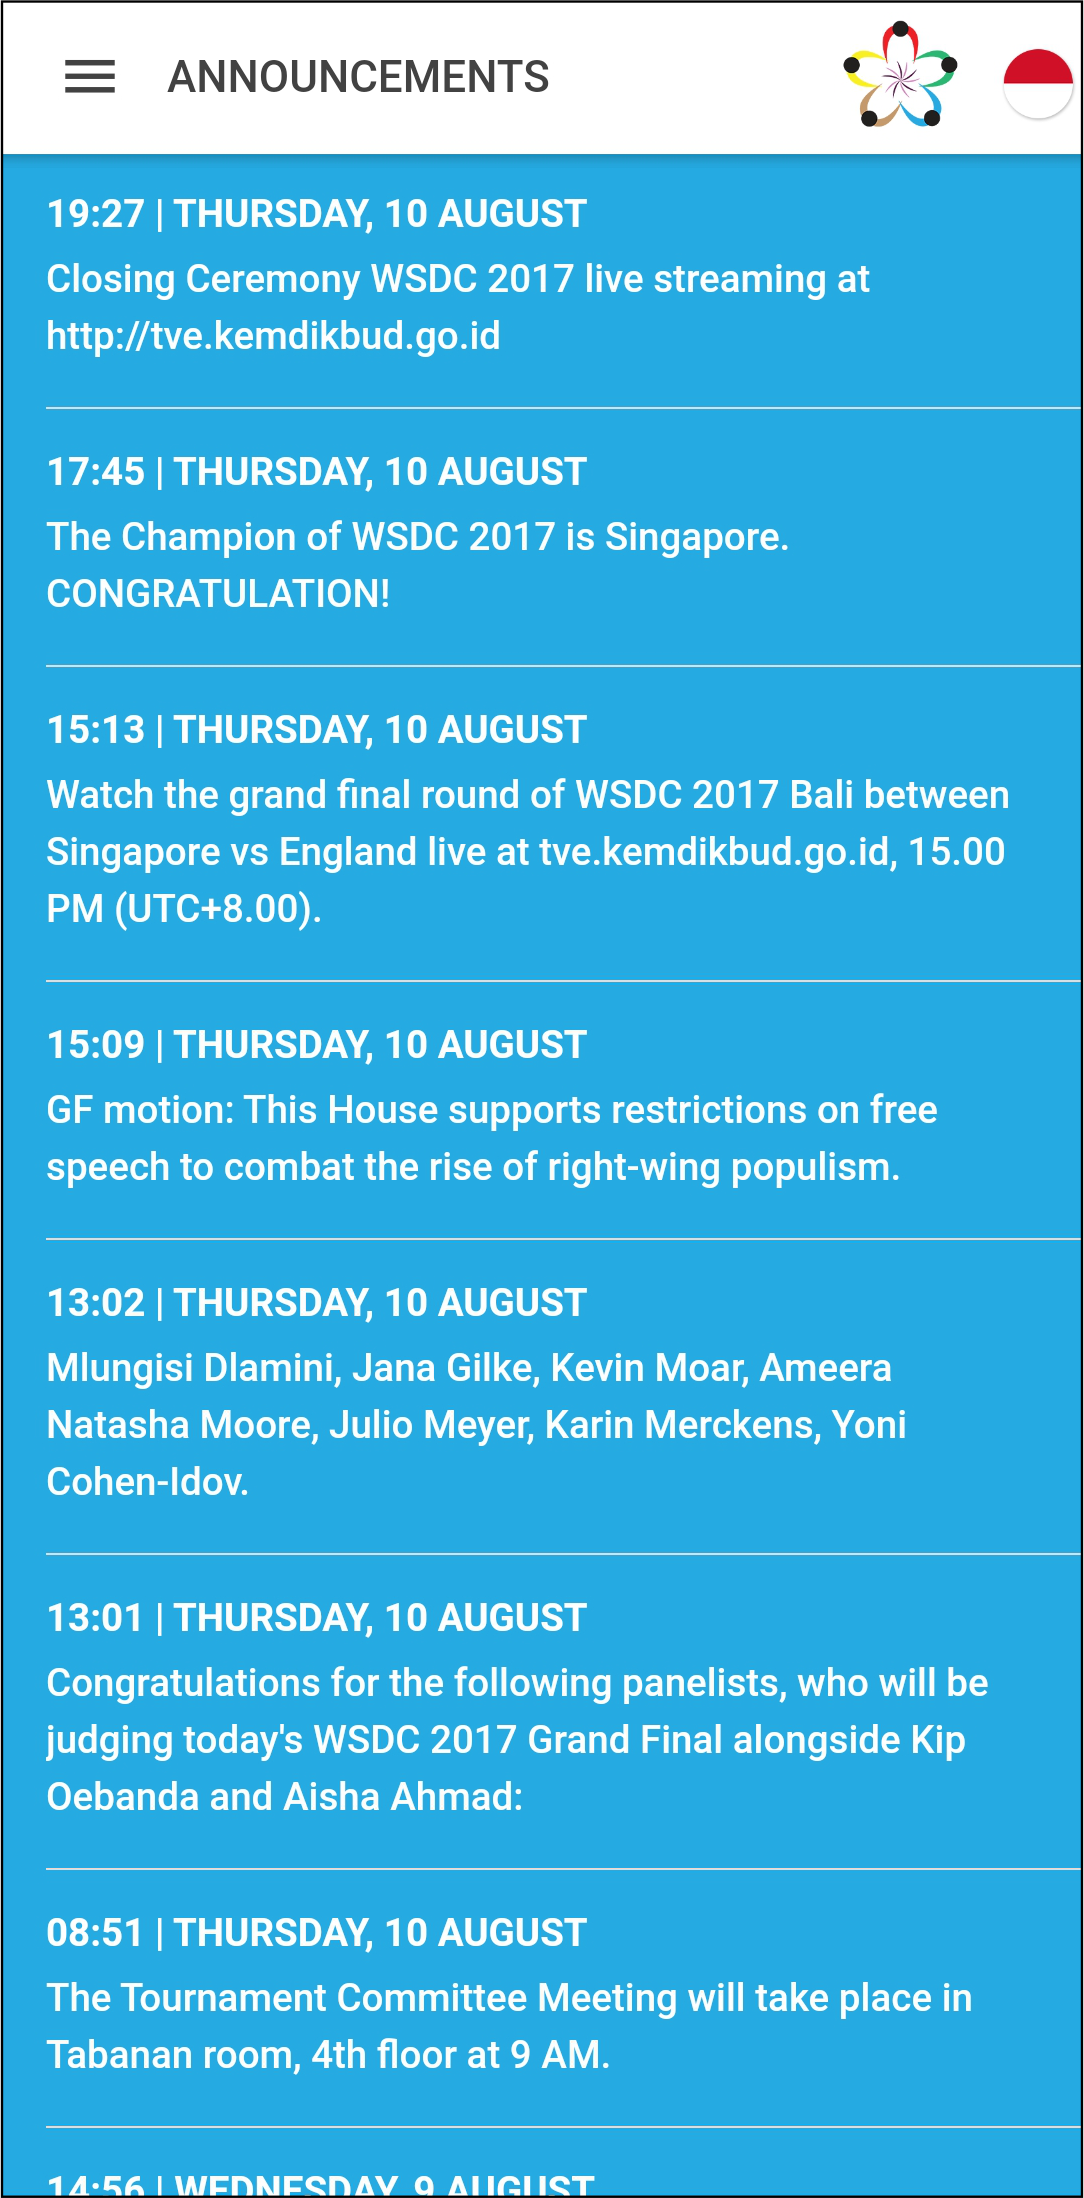
\includegraphics[scale=0.4]{Gambar/AnnouncementsPage.png}
	    \caption{Halaman {\it Announcements}}
	    \label{fig:wsdcAppAnnouncements}
     \end{subfigure}
     \hfill
     \begin{subfigure}[b]{0.3\textwidth}
         \centering
	    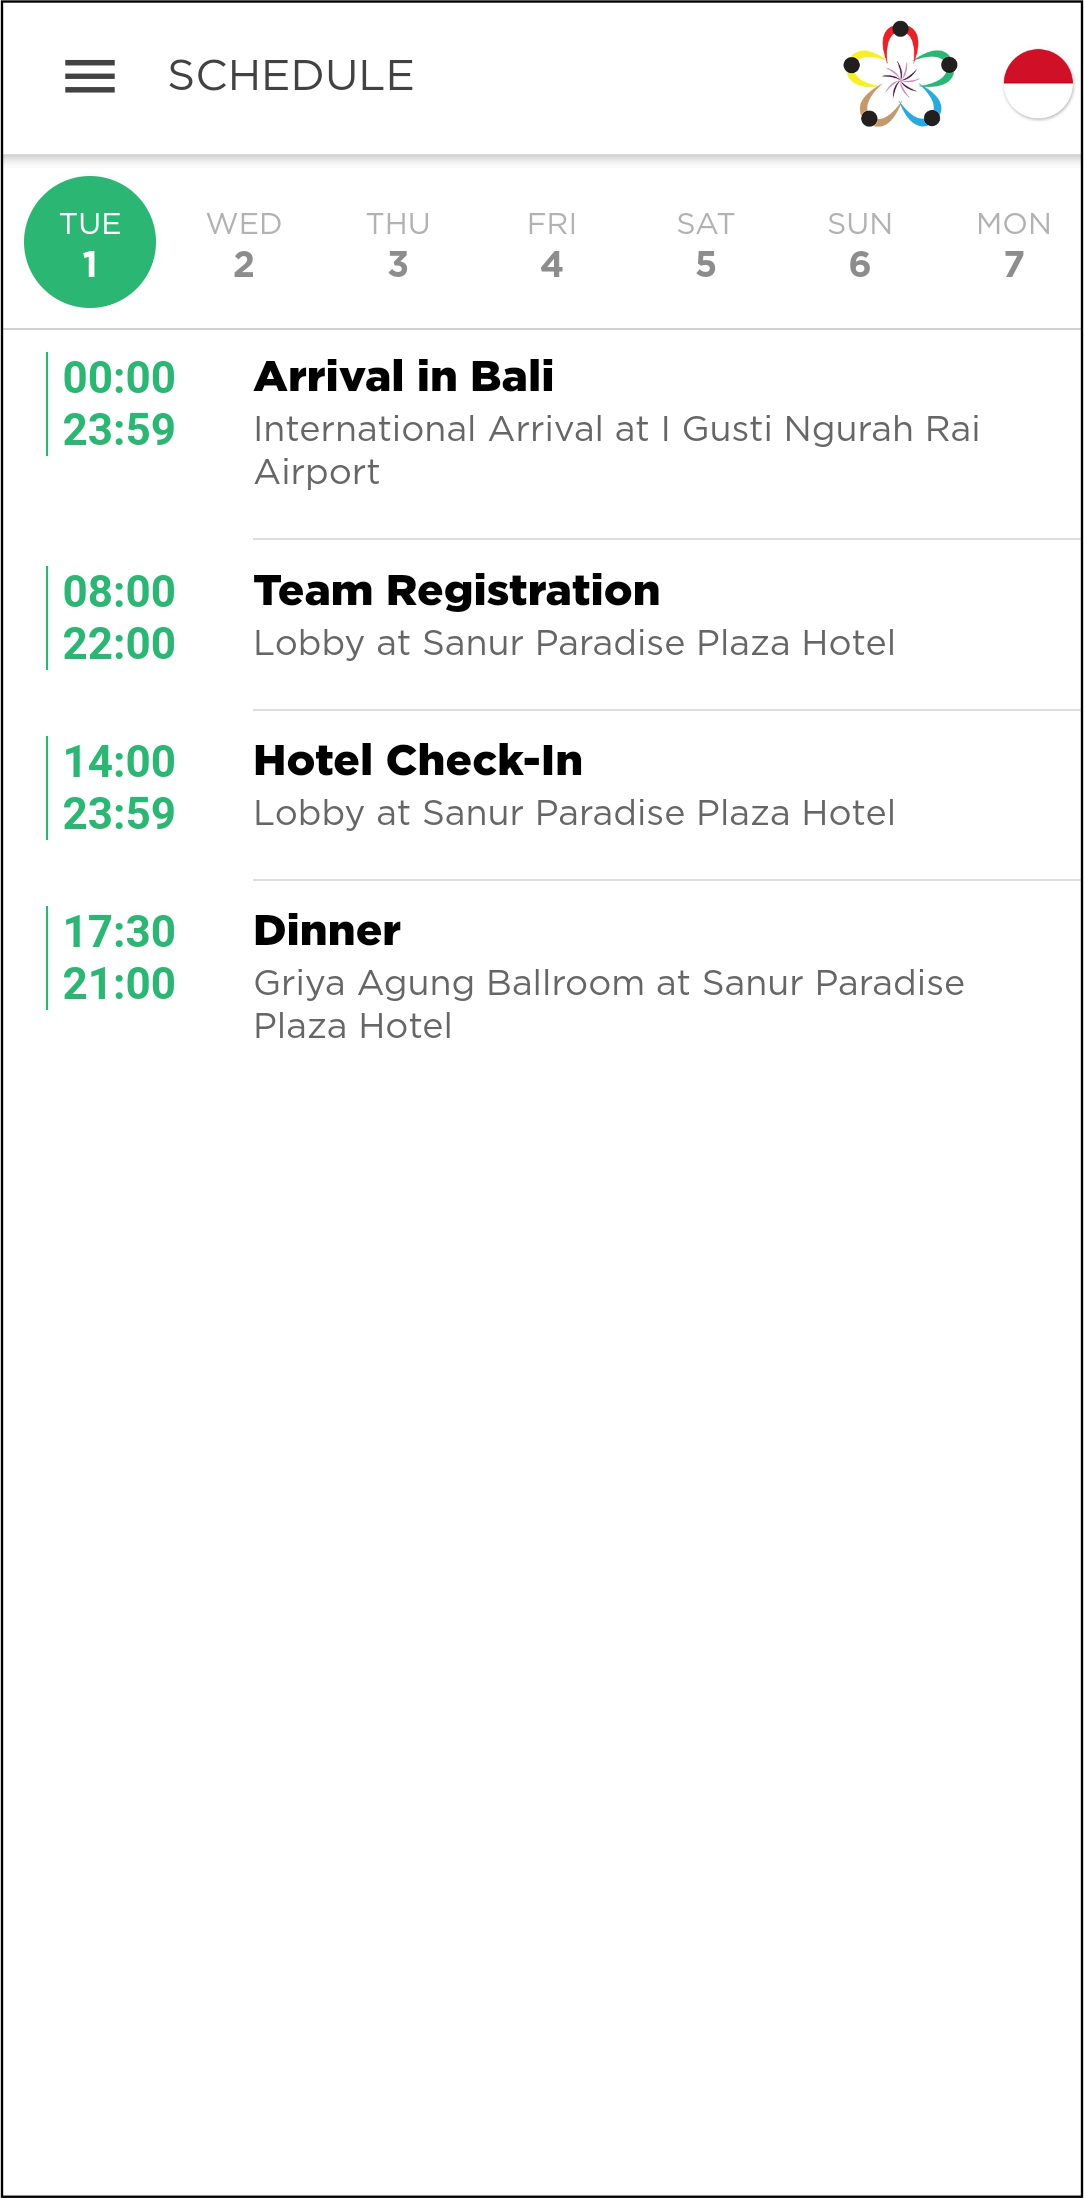
\includegraphics[scale=0.4]{Gambar/SchedulePage.png}
	    \caption{Halaman {\it Schedule}}
	    \label{fig:wsdcAppSchedule}
     \end{subfigure}
        \caption{Aplikasi WSDC 2017 Bali Saat Ini pada Perangkat Android}
        \label{fig:three graphs}
\end{figure}

Fitur-fitur yang terdapat di aplikasi WSDC 2017 Bali saat ini yaitu :

\begin{enumerate}
	\item {\it Newsletter} : Pengguna dapat mengunduh dan berita-berita terkait acara WSDC 2017 Bali (Gambar~\ref{fig:wsdcapp}).

	\item {\it Announcements} : Pengguna dapat melihat pemberitahuan tentang berjalannya acara WSDC 2017 Bali (Gambar~\ref{fig:wsdcAppAnnouncements}).

	\item {\it Schedule} : Pengguna dapat melihat jadwal acara WSDC 2017 Bali yang sudah diadakan (Gambar~\ref{fig:wsdcAppSchedule}).

	\item {\it Venues} : Pengguna dapat melihat berbagai macam lokasi acara WSDC 2017 Bali, mulai dari lokasi upacara, lokasi kompetisi, dan lokasi wisata edukasi. Masing-masing dari lokasi tersebut dapat menunjukan arah dan jarak dari lokasi tempat pengguna berada (Gambar~\ref{fig:wsdcAppVenues}).

	\item Info : Pengguna dapat melihat informasi terkait dengan tim pengembang dari aplikasi WSDC 2017 Bali, kontak-kontak penting yang dapat dihubungi, dan kosa kata penting dalam Bahasa Indonesia (Gambar~\ref{fig:wsdcAppInfo}).

	\item {\it Draw} : Pengguna dapat melihat melihat pembagian {\it venue} dan kubu proposisi atau oposisi dari hasil pengundian untuk para negara peserta WSDC 2017 Bali (Gambar~\ref{fig:wsdcAppDraw}).

	\item {\it Result} : Pengguna dapat melihat informasi terkait hasil dari pertandingan pada semi final, perempat final, dan perdelapan final WSDC 2017 Bali (Gambar~\ref{fig:wsdcAppResult}).
\end{enumerate}

\begin{figure}[H]
     \centering
     \begin{subfigure}[b]{0.21\textwidth}
        \centering
	    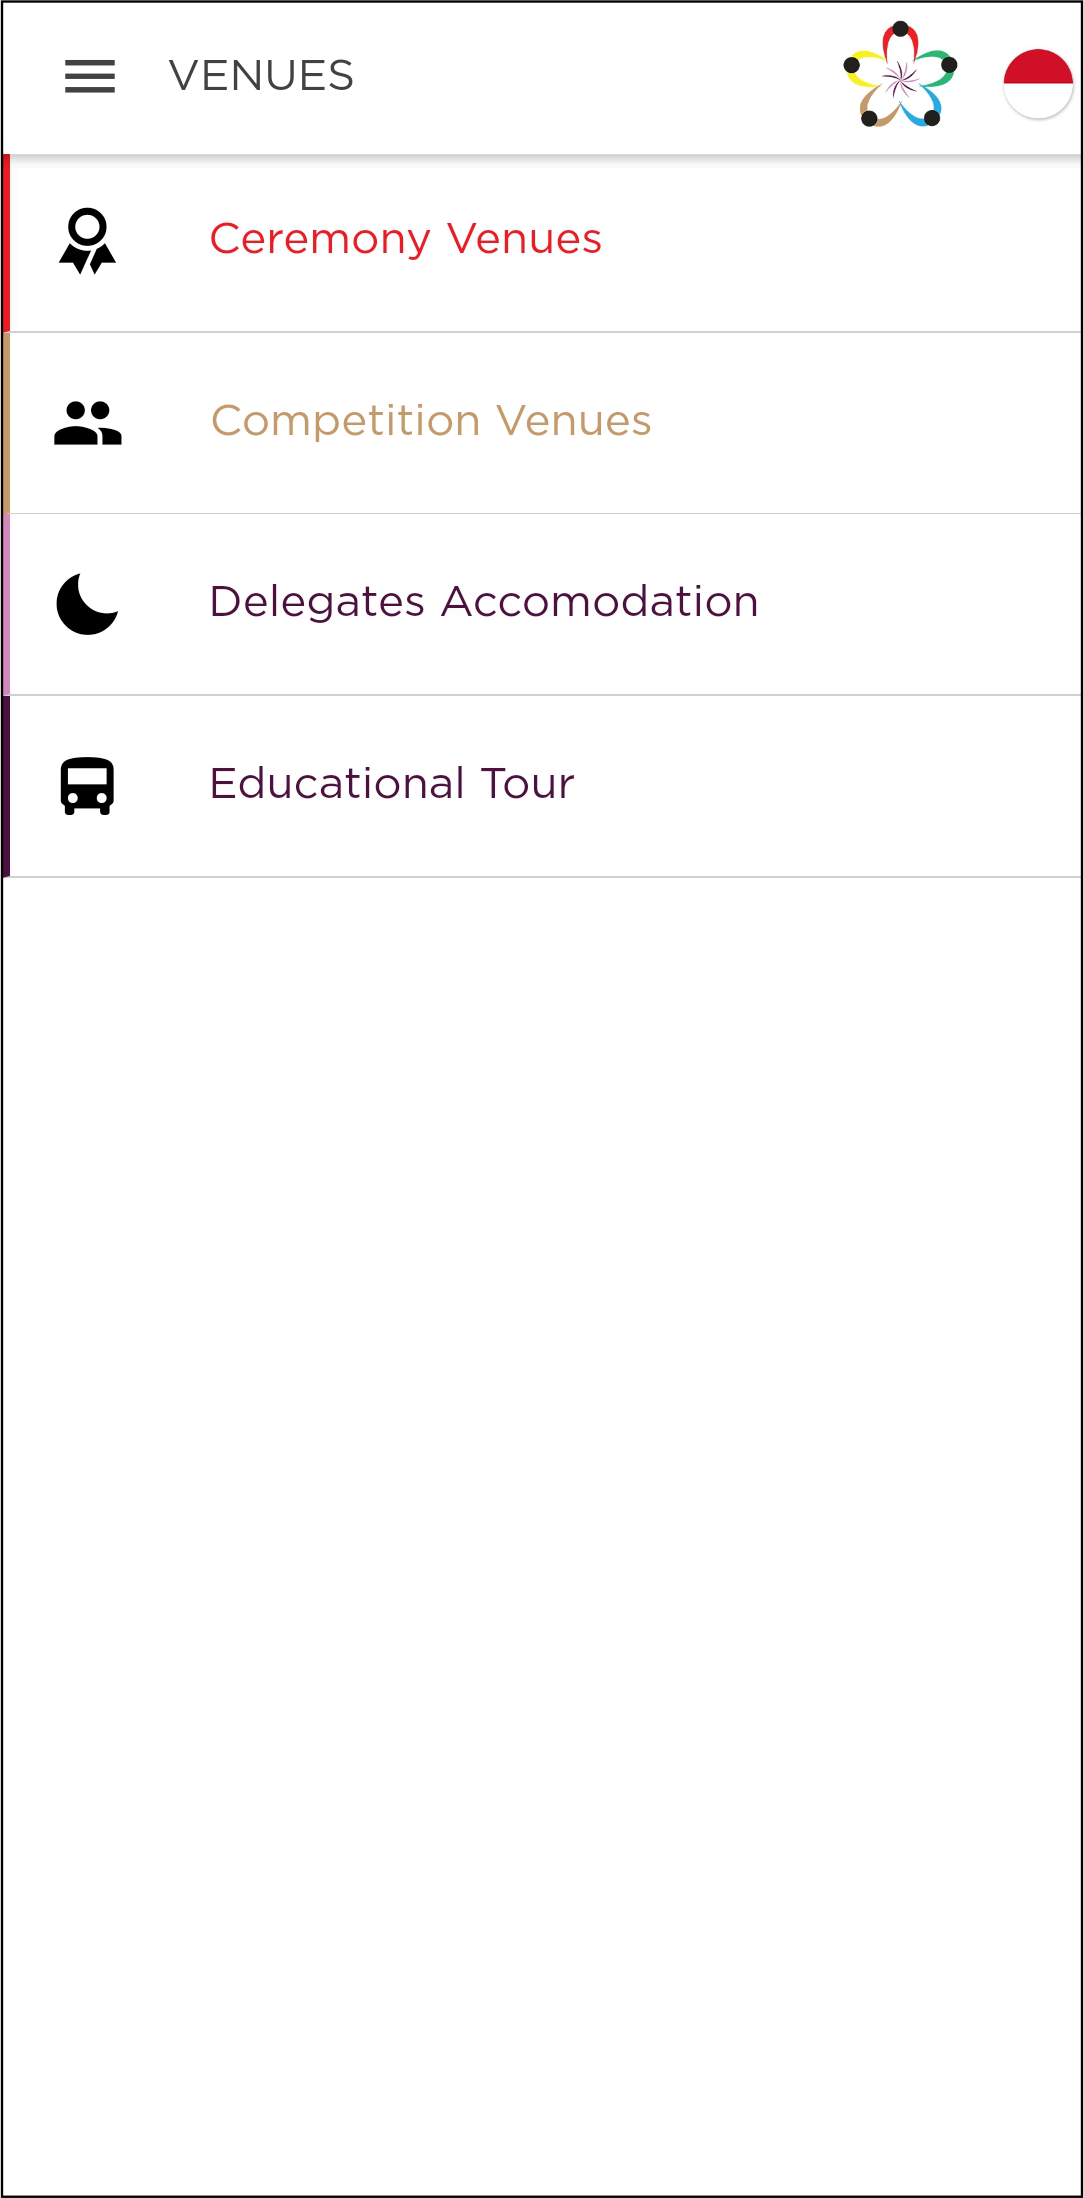
\includegraphics[scale=0.4]{Gambar/VenuePage.png}
	    \caption{Halaman {\it Venues}}
	    \label{fig:wsdcAppVenues}
     \end{subfigure}
     \hfill
     \begin{subfigure}[b]{0.247\textwidth}
    \centering
	    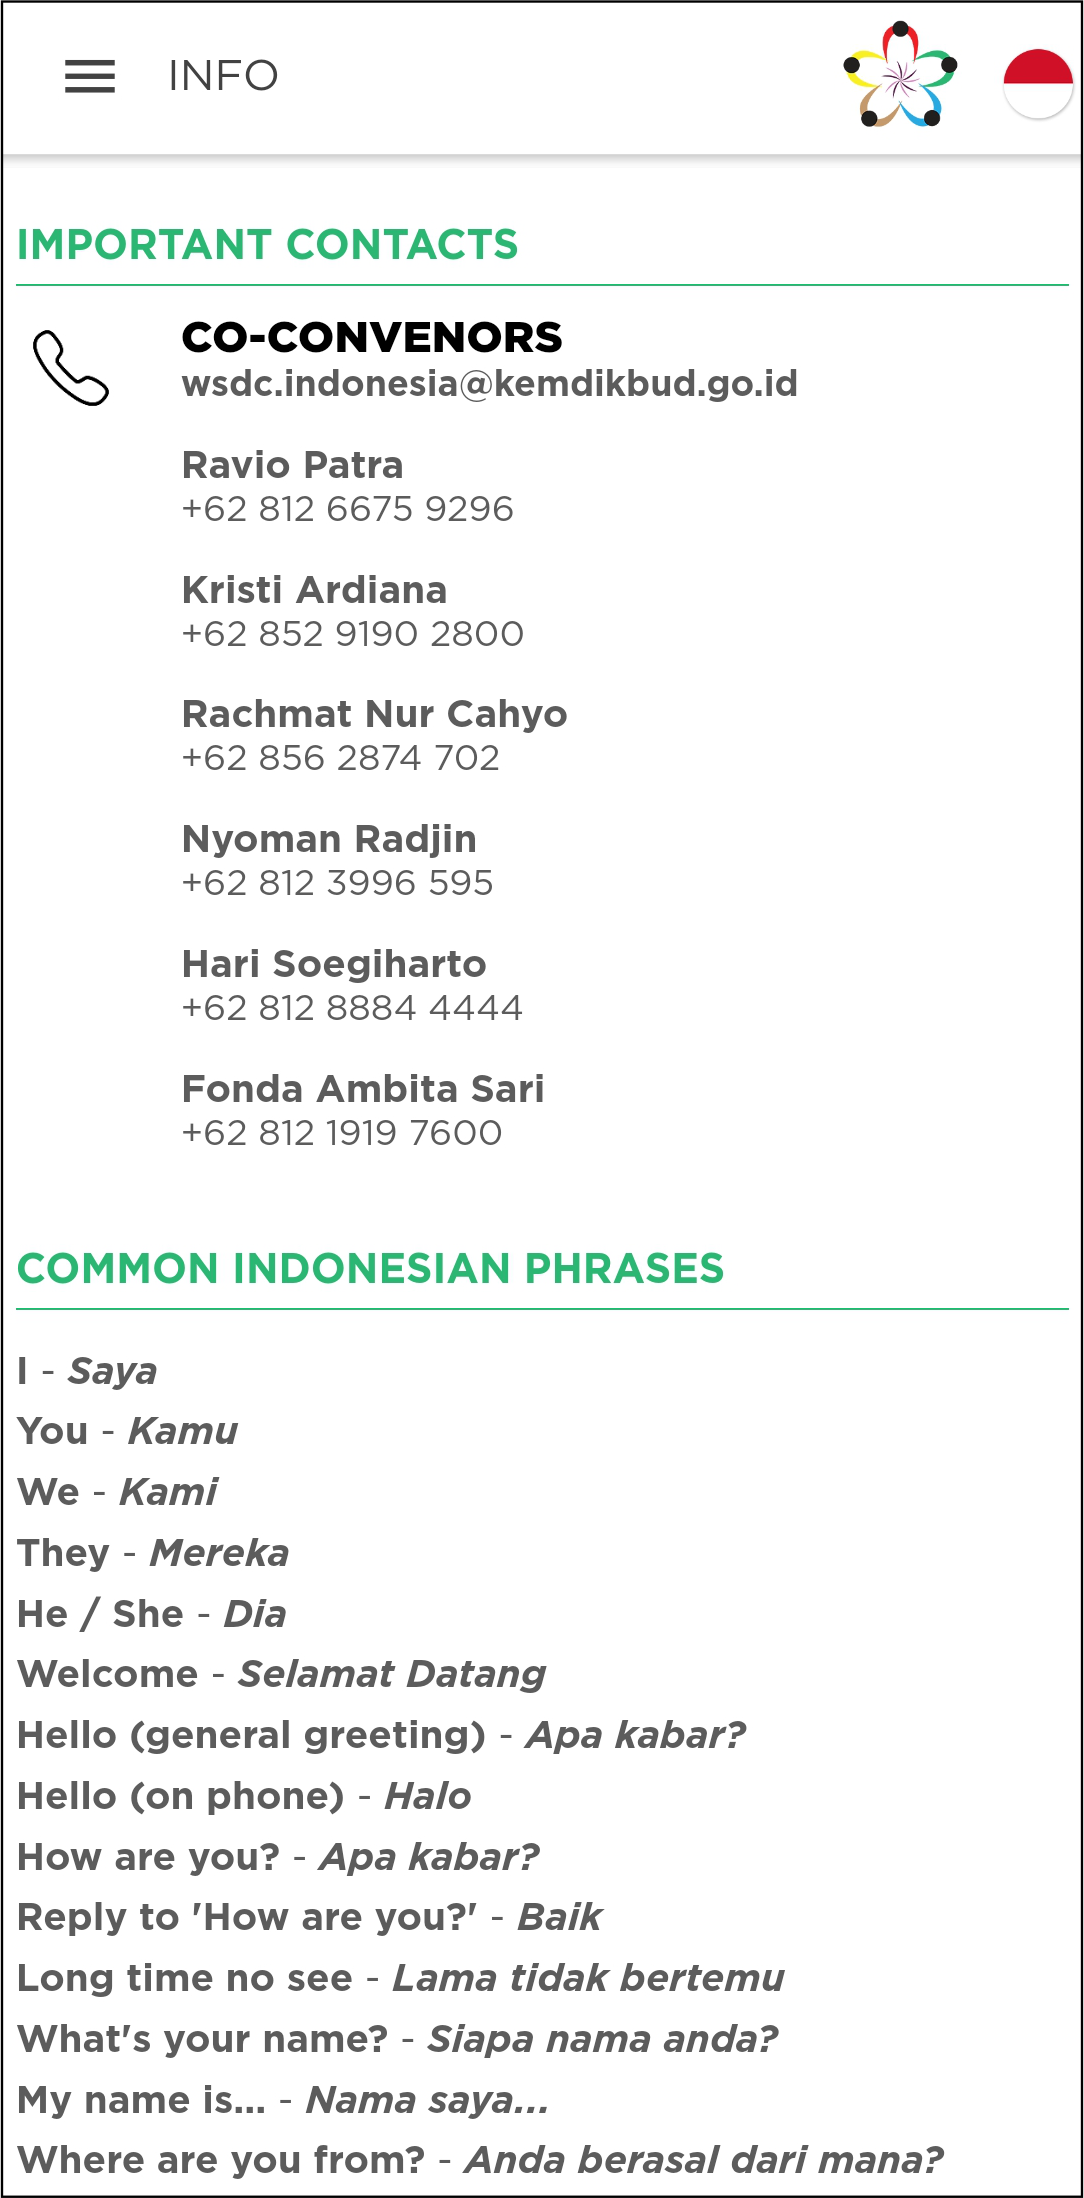
\includegraphics[scale=0.4]{Gambar/InfoPage.png}
	    \caption{Halaman Info}
	    \label{fig:wsdcAppInfo}
     \end{subfigure}
	\begin{subfigure}[b]{0.247\textwidth}
    \centering
	    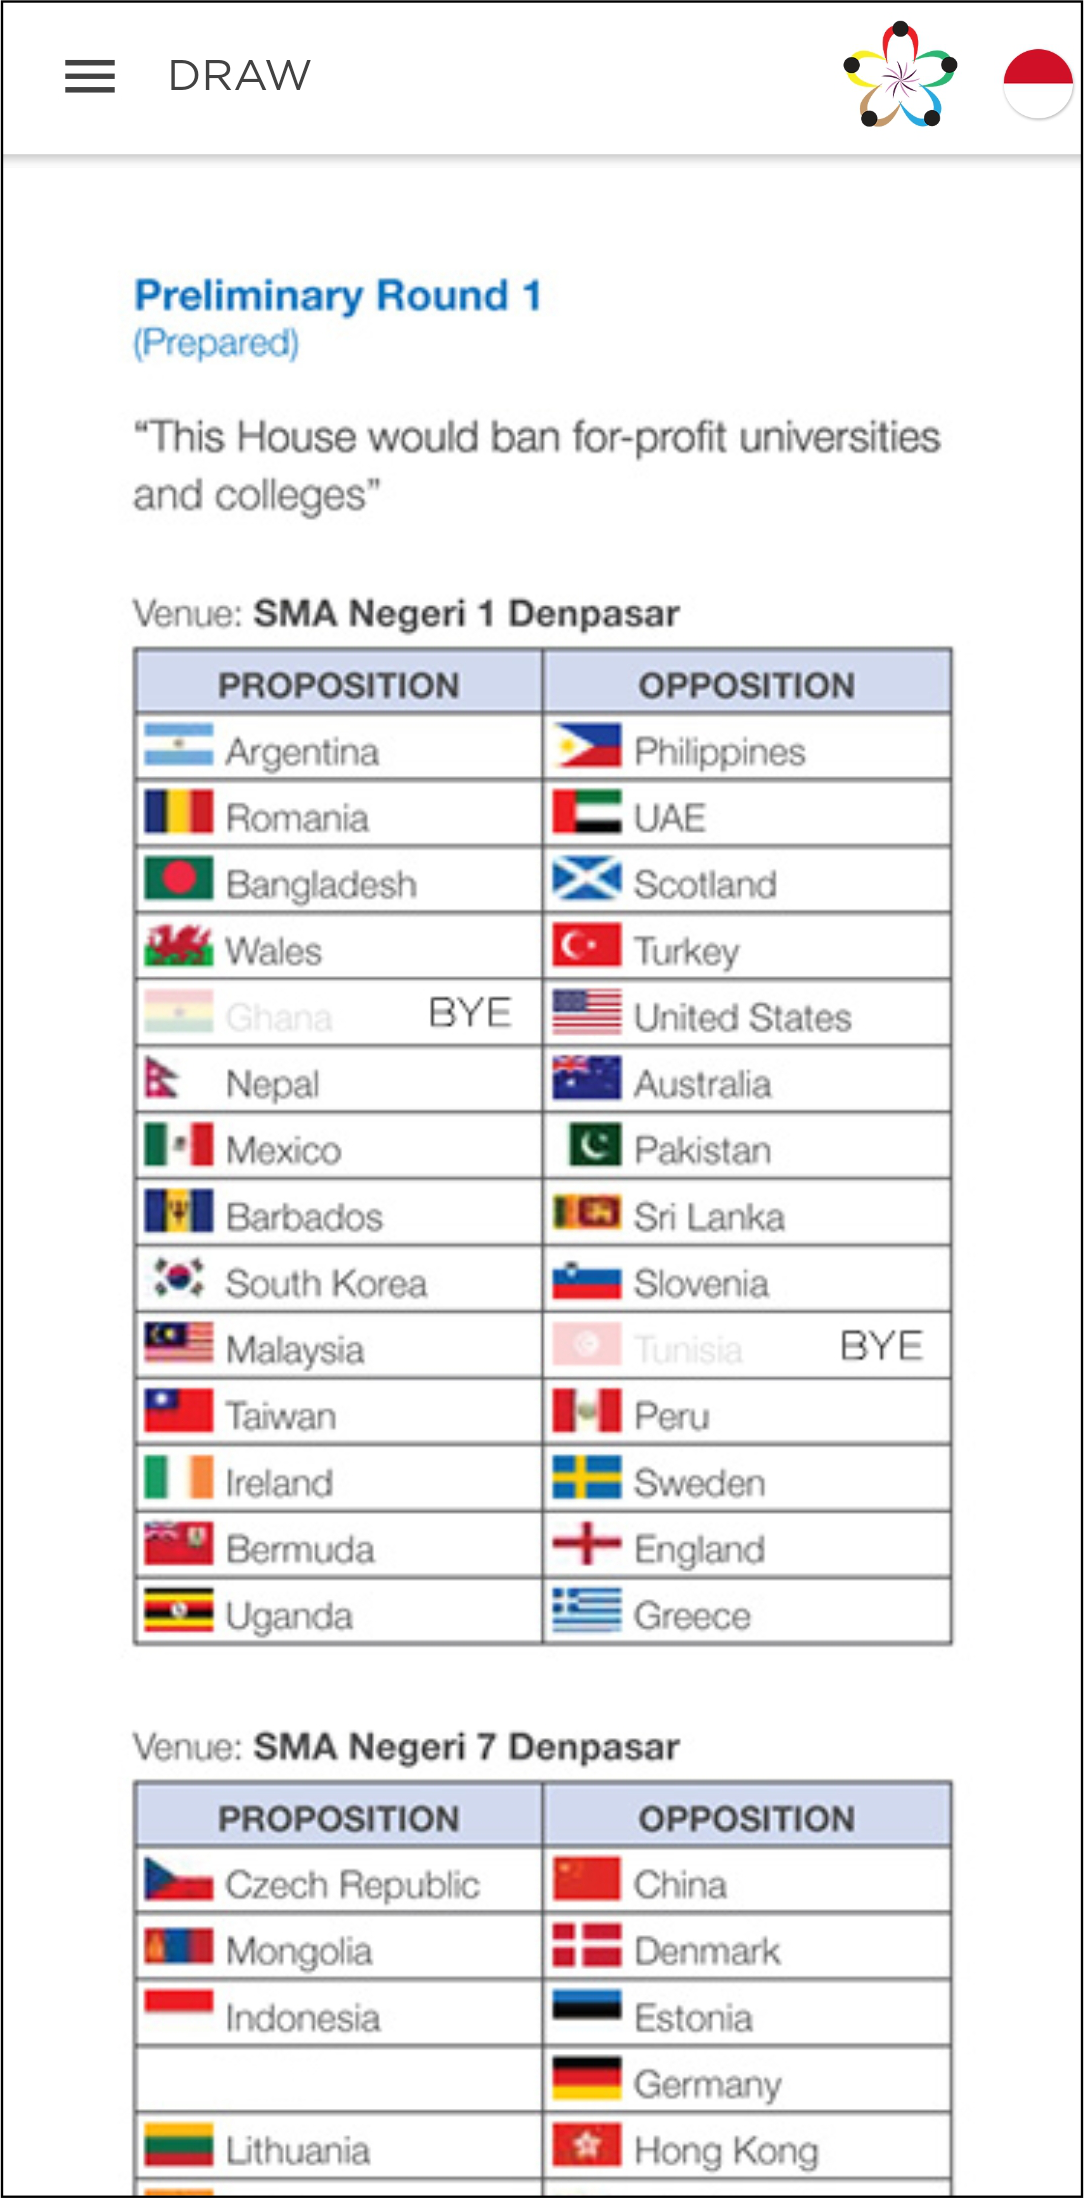
\includegraphics[scale=0.4]{Gambar/DrawPage.png}
	    \caption{Halaman {\it Draw}}
	    \label{fig:wsdcAppDraw}
     \end{subfigure}
	\begin{subfigure}[b]{0.247\textwidth}
    \centering
	    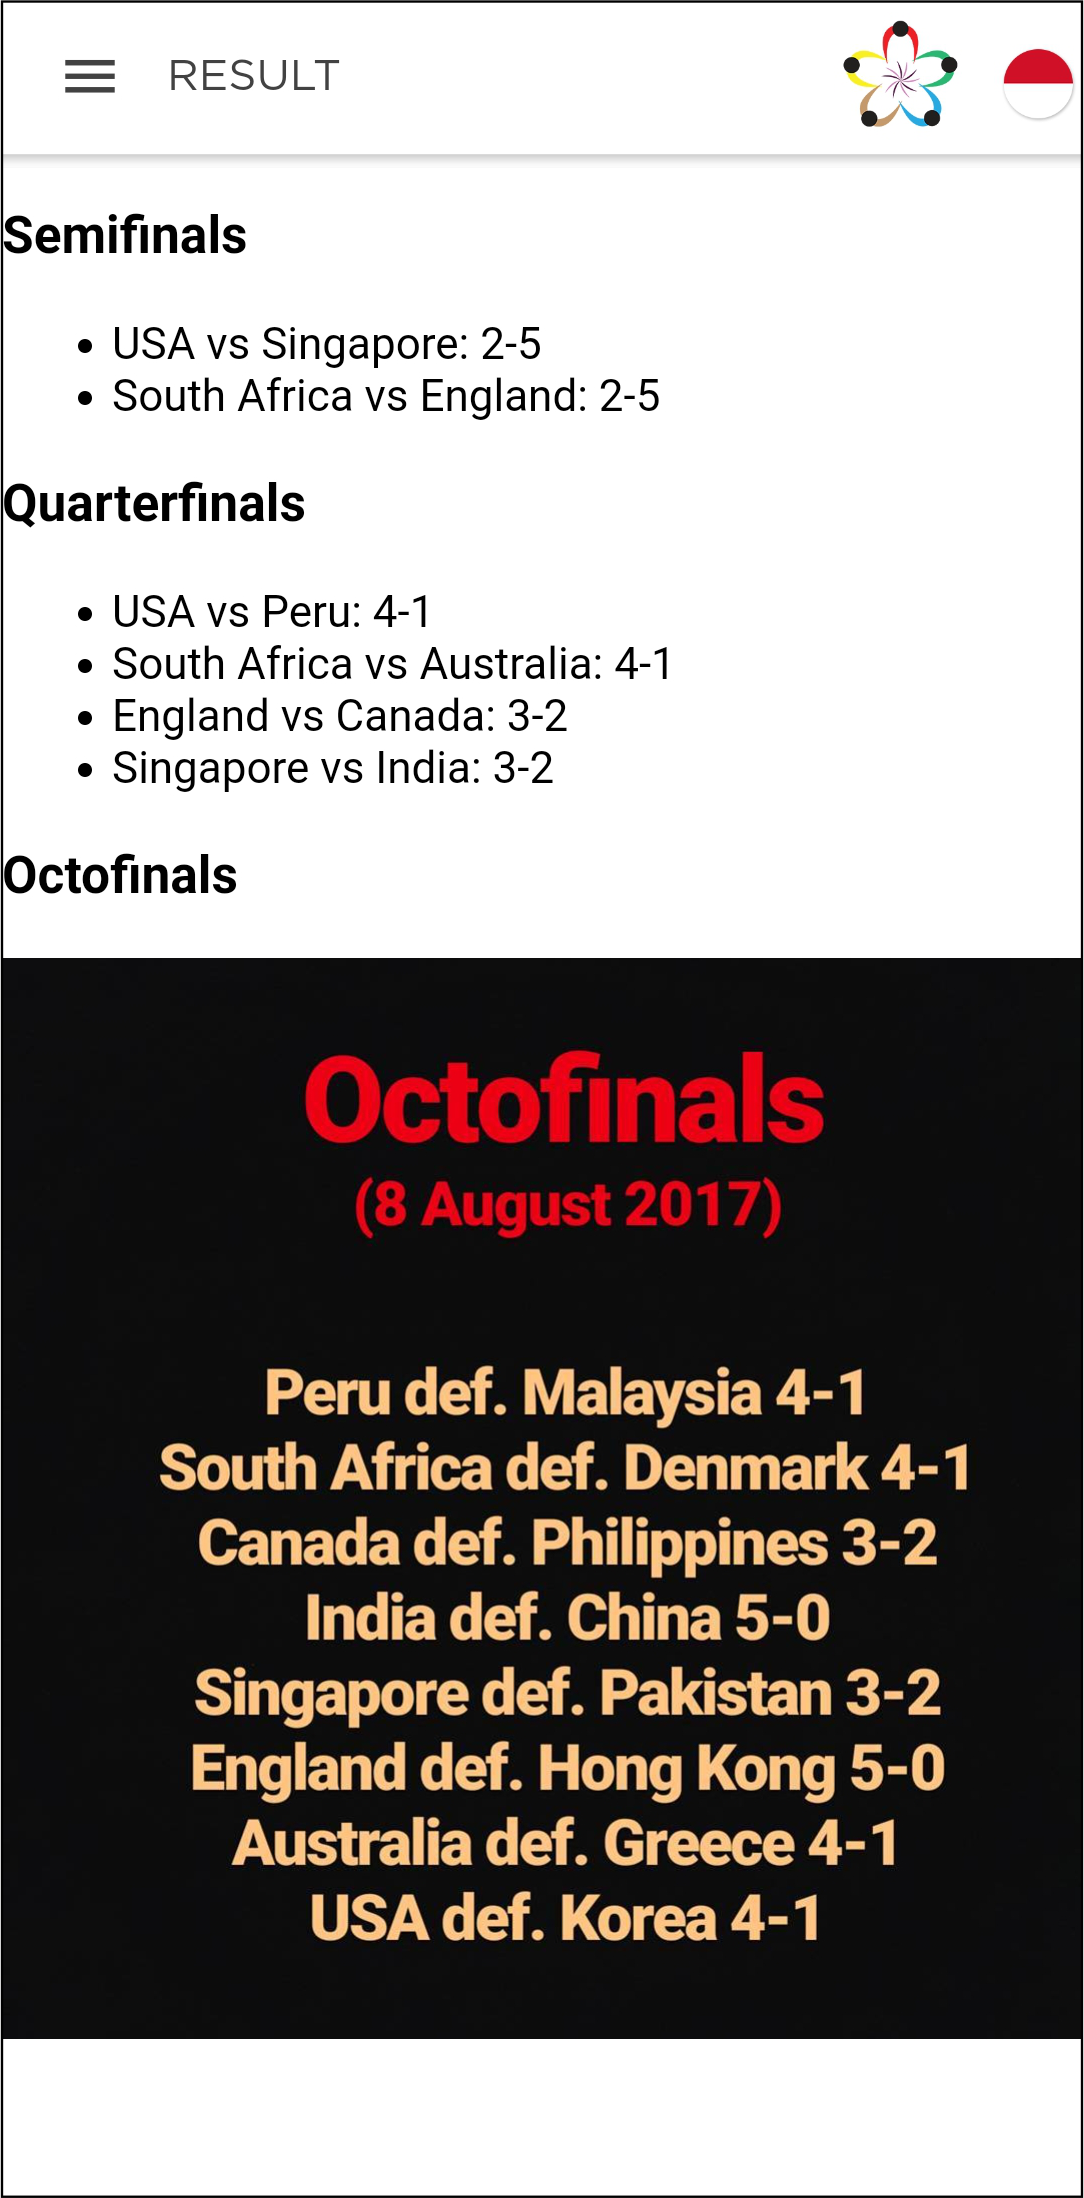
\includegraphics[scale=0.4]{Gambar/ResultPage.png}
	    \caption{Halaman {\it Result}}
	    \label{fig:wsdcAppResult}
     \end{subfigure}
	\caption{Aplikasi WSDC 2017 Bali Saat Ini pada Perangkat Android}
        \label{fig:three graphs}
\end{figure}



\section{Ionic Framework}
\label{sec:ionicframework} 
 
Ionic Framework merupakan sebuah kerangka kerja {\it open source} lintas platform yang memungkinkan untuk mengembangkan aplikasi hibrida yang bekerja pada berbagai macam platform seluler seperti {\it android}, iOS, dan Windows~\cite{waranashiwar:18:ionic}. Ionic memiliki berbagai macam \textit{front-end library} dan komponen \textit{User Interface}(UI) yang digunakan untuk  perancangan aplikasi menggunakan teknologi web seperti HTML, CSS, dan Javascript, dengan integrasi untuk berbagai \textit{framework} seperti Angular, React, dan Vue. Saat pertama kali dibuat, Ionic menggunakan AngularJS. Namun, seiring saat Angular versi 2 yang menggunakan Typescript dirilis, Ionic versi 2 dan selanjutnya menggunakan Angular. Lalu, pada tahun 2019, Ionic mendukung penggunaan \textit{framework} lain selain Angular, yaitu React dan Vue. Di dalam Ionic, Angular digunakan untuk membangun aplikasi dan perutean, sehingga aplikasi dapat sejalan dengan ekosistem Angular lainnya. Ionic menyediakan {\it toolkit} Angular untuk membangun aplikasi dan terintegrasi dengan Angular CLI resmi yang menyediakan fitur khusus untuk aplikasi Ionic Angular. Pada saat skripsi ini dibuat, Ionic versi terbaru adalah Ionic versi 5, sedangkan Angular yang digunakan adalah Angular versi 12. 

\subsection{Native API}
\label{subsec:nativeApi}
Native API memungkinkan pengembangan aplikasi langsung terintegrasi ke dalam platform. Pengembang dapat membuat aplikasi pada perangkat {\it mobile} untuk dapat diimplementasikan ke berbagai {\it platform}, seperti IOS dan Android, setelah pengembangan selesai di dalam {\it framework native} tanpa perlu perubahan, dan tidak mempengaruhi peforma dari aplikasi tersebut~\cite{griffith:17:mobile}. 

Ionic mendukung komunikasi dengan menggunakan Native API yang terintegrasi untuk menambahkan fungsionalitas ke dalam aplikasi Ionic apapun dengan menggunakan Capacitor atau Cordova. Dengan terpasangnya Ionic Native, maka aplikasi akan memiliki antar muka yang diperlukan untuk berinteraksi dengan salah satu {\it plug-in}, yaitu Capacitor atau Cordova.

\subsubsection{Capacitor}
\label{subsec:capacitor}
Tujuan dari Capacitor adalah untuk menyediakan akses ke perangkat {\it native} dan fitur platform, serta untuk menyediakan satu set API untuk mengembangkan aplikasi seluler secara hibrida, {\it Progressive Web Apps} berbasis web, dan aplikasi komputer berbasis Electron~\cite{tor:19:software}. Capacitor merupakan penerus dari Cordova, dengan tujuan untuk memungkinkan aplikasi web modern berjalan di semua platform utama. Capacitor juga mendapat dukungan terhadap banyak {\it plugi-n} Cordova.

\subsubsection{Cordova}
\label{subsec:cordova}
Cordova merupakan {\it framework open source} yang dapat membuat pengembang untuk menggunakan teknologi seperti HTML, JavaScript, dan CSS untuk membangun aplikasi untuk perangkat bergerak yang dapat berjalan pada beberapa sistem operasi {\it mobile}~\cite{gonsalves:18:evaluating}. Cordova menyediakan antarmuka antara WebView dan lapisan {\it native} pada perangkat~\cite{griffith:17:mobile}. Selain dapat bekerja pada dua platform seluler Android dan IOS, Cordova juga dapat digunakan pada platform seluler seperti Windows Phone, Blackberry, dan FireOS.

Untuk mengonfigurasi proyek Cordova, saat ini dapat menggunakan {\it Command Line Tool} (CLI). CLI membuat proyek dasar dan mengonfigurasinya agar berfungsi dengan platform seluler apa pun yang didukung yang dapat digunakan. Cordova CLI juga dapat membuat pengembang memliki integrasi dan pengelolaan {\it plug-in}. Selain itu, CLI juga dapat mengkompilasi aplikasi untuk berjalan pada simulator atau pada perangkat {\it native}. Serupa dengan Capacitor, Cordova membuat pengembang dapat mengakses fitur {\it native} dari sebuah perangkat, seperti kamera, papan ketik, dan geolokasi, menggunakan {\it plugin}. {\it Framework} Ionic telah terdapat berbagai macam TypeScript {\it wrapper} untuk {\it plugins} Cordova.  Untuk dapat menggunakan Cordova Plugins, yaitu dengan memasang Cordova Plugins terlebih dahulu (Kode~\ref{lst:installCordova}), dan memperbaruinya ke versi terakhir (Kode~\ref{lst:updateCordova}) yang dapat dilakukan melalui CLI. Setiap {\it plugins} memiliki dua komponen, yaitu kode {\it native} (Cordova), dan kode TypeScript (Ionic Native). Cordova Plugins juga dibungkus di dalam Promise atau Observable untuk menyediakan antarmuka {\it plug-in}.

\begin{lstlisting}[language=html, label={lst:installCordova}, caption=Kode untuk Memasang Cordova Plugins]
npm install cordova-plugin-name
npx cap sync
\end{lstlisting} 

\begin{lstlisting}[language=php, label={lst:updateCordova}, caption=Kode untuk Memperbarui Cordova Plugins]
npm install cordova-plugin-name@2
npx cap update
\end{lstlisting} 


\subsection{UI Component}
\label{subsec:uiComponent}
{\it Framework} Ionic menggunakan kemampuan Angular dalam memperluas kosakata HTML, yaitu menyertakan {\it tag} khusus untuk menciptakan seluruh rangkaian komponen~\cite{griffith:17:mobile}. Semua komponen memiliki awalan ion, sehingga dapat dikenali dalam markup. Sama seperti {\it tag} HTML standar, komponen Ionic juga dapat menerima berbagai macam atribut sebagai pengaturan dari {\it tag} tersebut, seperti mengatur id atau mendefinisikan kelas CSS tambahan. Terdapat beberapa komponen yang ada pada {\it framework} Ionic yaitu :
\begin{itemize}
	\item Action Sheet \\
	Merupakan dialog yang menampilkan serangkaian opsi, yang muncul di atas konten aplikasi dan harus ditutup secara manual oleh pengguna sebelum pengguna dapat melanjutkan interaksi dengan aplikasi. Untuk menutup Action Sheet terdapat beberapa cara, termasuk mengetuk latar belakang atau menekan tombol escape di desktop.

	\item Alert \\
	Alert merupakan dialog yang menampilkan informasi kepada pengguna, atau mengumpulkan informasi dari pengguna menggunakan input. Alert muncul di atas konten aplikasi, dan harus ditutup secara manual oleh pengguna sebelum pengguna dapat melanjutkan interaksi dengan aplikasi. Secara opsional, terdapat header, sub header, dan pesan yang ada pada Alert.
	\item Badge \\
	Merupakan elemen {\it inline block} yang biasanya muncul di dekat elemen lain, berisi angka atau karakter lain, yang digunakan sebagai pemberitahuan bahwa ada item tambahan yang terkait dengan suatu elemen dan menunjukan berapa banyak item yang ada. Penggunaan Badge dengan menggunakan {\it tag} <ion-badge> (Kode~\ref{lst:badgeComponent}).
	\begin{lstlisting}[language=php, label={lst:badgeComponent}, caption=Potongan Kode Program dari Badge Component]
<ion-badge>99</ion-badge>
	\end{lstlisting} 
	\item Button \\
	Merupakan elemen yang dapat diklik, biasanya digunakan dalam formulir atau di mana pun yang membutuhkan fungsionalitas tombol. Button biasanya menampilkan teks, ikon, atau bisa juga keduanya. Button dapat pula menggunakan atribut untuk menampilkannya dengan penampilan tertentu. Penggunaan Button dengan menggunakan {\it tag} <ion-button>  (Kode~\ref{lst:buttonComponent}). \newpage
	\begin{lstlisting}[language=php, label={lst:buttonComponent}, caption=Potongan Kode Program dari Button Component]
<ion-button>Default</ion-button>
	\end{lstlisting} 

	\item Card \\
	Merupakan bagian standar dari tampilan antarmuka yang berfungsi sebagai titik masuk ke dalam informasi yang lebih detail. Card dapat menjadi satu komponen, tetapi sering kali terdiri dari beberapa header, judul, sub judul, dan konten. Penggunaan Card dengan menggunakan {\it tag} <ion-card> yang dapat berisi {\it header}, {\it subtitle}, {\it title}, dan {\it content} (Kode~\ref{lst:cardComponent}).
	\begin{lstlisting}[language=php, label={lst:cardComponent}, caption=Potongan Kode Program dari Card Component]
<ion-card>
	<ion-card-header>
		<ion-card-subtitle>Card Subtitle</ion-card-subtitle>
		<ion-card-title>Card Title</ion-card-title>
	</ion-card-header>
				
	<ion-card-content>
		Card Content
	</ion-card-content>
</ion-card>
	\end{lstlisting} 
	\item Content\\
	Komponen content merupakan penyedia area konten yang bisa digunakan untuk mengontrol area yang dapat digulir. Dalam satu tampilan, setidaknya terdapat satu buah content. Content juga dapat dimodifikasi padding, margin, dan lainnya menggunakan {\it global style} yang berada di CSS Utilites atau mengubahnya secara individual dengan menggunakan CSS. Penggunaan Content dengan menggunakan {\it tag} <ion-content> (Kode~\ref{lst:contentComponent}).

	\begin{lstlisting}[language=php, label={lst:contentComponent}, caption=Potongan Kode Program dari Content Component]
<ion-content
	[scrollEvents]="true"
	(ionScrollStart)="logScrollStart()"
	(ionScroll)="logScrolling($event)"
	(ionScrollEnd)="logScrollEnd()">
		<h1>Main Content</h1>
			
			<div slot="fixed">
				<h1>Fixed Content</h1>
			</div>
</ion-content>
	\end{lstlisting} 
	\item Date and Time Pickers\\
	Datetime merupakan penampil antarmuka untuk pengguna memilih tanggal dan waktu. Terdapat kolom yang dapat digulir yang dapat digunakan untuk memilih tahun, bulan, hari, jam, dan menit secara individual. Komponen ini menampilkan nilai di dua tempat, yaitu di komponen <ion-datetime> (Kode~\ref{lst:datetimeComponent}), dan di antarmuka pemilih yang ditampilkan dari bawah layar.
		\begin{lstlisting}[language=php, label={lst:datetimeComponent}, caption=Kode Program dari Datetime Component dengan Format Bulan-Hari-Tahun]
<ion-datetime displayFormat="MM DD YY" placeholder="Select Date"></ion-datetime>
		\end{lstlisting} 
	\item Infinite Scroll	\\
	Komponen Infinite Scroll memanggil sebuah action yang akan dilakukan ketika pengguna menggulir dengan jarak tertentu dari bawah atau atas halaman. Penggunaan Infinite Scroll dengan menggunakan {\it tag} <ion-infinite-scroll> (Kode~\ref{lst:InfiteScrollComponent}). 
	\begin{lstlisting}[language=php, label={lst:InfiteScrollComponent}, caption=Potongan Kode Program dari Infinite Scroll Component]
<ion-infinite-scroll threshold="100px" (ionInfinite)="loadData($event)">
	<ion-infinite-scroll-content
		loadingSpinner="bubbles"
		loadingText="Loading more data...">
	</ion-infinite-scroll-content>
</ion-infinite-scroll>
	\end{lstlisting} 
	\item Item \\
	Item merupakan elemen yang dapat berisi teks, ikon, avatar, gambar, masukan, dan elemen asli atau kustom lainnya. Biasanya, item ditempatkan di dalam sebuah {\it list} bersamaan dengan item lainnya dengan {\it tag} <ion-item> (Kode~\ref{lst:itemComponent}). Dapat dilakukan {\it swipe}, dihapus, disusun ulang, dan diedit.
	\begin{lstlisting}[language=php, label={lst:itemComponent}, caption=Potongan Kode Program dari Item Component]
<ion-item>
	<ion-label>
		Item
	</ion-label>
</ion-item>
	\end{lstlisting} 
	\item Menu \\
	Komponen menu merupakan panel navigasi samping yang dapat dilakukan {\it slides} dari sisi pada tampilan halaman saat ini menggunakan {\it tag} <ion-menu> (Kode~\ref{lst:menuComponent}). Pada dasarnya, Menu muncul dari kiri, tetapi sisi kemunculan menu dapat diganti. 

	\begin{lstlisting}[language=php, label={lst:menuComponent}, caption=Potongan Kode Program dari Menu Component]
<ion-menu side="start" menuId="first" contentId="main">
	<ion-header>
		<ion-toolbar color="primary">
			<ion-title>Start Menu</ion-title>
		</ion-toolbar>
	</ion-header>
	<ion-content>
		<ion-list>
			<ion-item>Menu Item</ion-item>
			<ion-item>Menu Item</ion-item>
			<ion-item>Menu Item</ion-item>
			<ion-item>Menu Item</ion-item>
			<ion-item>Menu Item</ion-item>
		</ion-list>
	</ion-content>
</ion-menu>
	\end{lstlisting} 
	\item Modal \\
	Modal merupakan kotak dialog yang muncul diatas konten aplikasi lain, dan harus diutup secara manual oleh pengguna sebelum pengguna dapat melanjutkan menggunakan aplikasi. Modal berguna sebagai komponen pilihan ketika ada banyak opsi untuk dipilih, atau melakukan penyaringan isi di dalam daftar, serta beberapa kasus serupa lainnya (Kode~\ref{lst:modalComponent}).
		\begin{lstlisting}[language=php, label={lst:modalComponent}, caption=Kode Program dari Modal]
import { Component, Input } from '@angular/core';

@Component({
	selector: 'modal-page',
})
export class ModalPage {	
	constructor() {}		
}
		\end{lstlisting} 
\newpage
	\item Navigation \\
	Navigation adalah komponen mandiri yang digunakan untuk membuat komponen baru ke dalam {\it stack}. Navigation tidak terikat kepada {\it router} tertentu, mengakibatkan jika kita membuat komponen Navigation dan melakukan {\it push} komponen lain ke dalam {\it stack}, komponen tersebut tidak akan mempengaruhi router aplikasi secara keseluruhan. Sesuai dengan kasus penggunaan dimana ketika pengguna bisa memilih modal, yang membutuhkan sub-navigasinya sendiri, tanpa membuatnya terikat ke URL aplikasi. 

	\item Segment \\
	Segment berfungsi untuk menampilkan pilihan tombol bagi pengguna untuk beralih di antara tampilan berbeda di dalam satu halaman yang sama. Segment menampilkan sekelompok tombol-tombol yang dapat diklik, dalam baris horizontal. Penggunaan Segment dengan menggunakan {\it tag} <ion-segment> (Kode~\ref{lst:segmentComponent}).
	\begin{lstlisting}[language=php, label={lst:segmentComponent}, caption=Kode Program dari Segment]
<ion-segment (ionChange)="segmentChanged($event)">
	<ion-segment-button value="friends">
		<ion-label>Friends</ion-label>
	</ion-segment-button>
	<ion-segment-button value="enemies">
		<ion-label>Enemies</ion-label>
	</ion-segment-button>
</ion-segment>
	\end{lstlisting}
	
	\item Tabs \\
	Tabs merupakan navigasi {\it top-level} yang mengimplementasi sebuah {\it tab-based navigation}. Tabs dapat digunakan dengan {\it tag} <ion-tabs> (Kode~\ref{lst:tabsComponent}) yang tidak memliki {\it styling} apapun dan bekerja sebagai {\it router outlet} untuk menangani navigasi. 
		\begin{lstlisting}[language=php, label={lst:tabsComponent}, caption=Kode Program dari Tabs]
<ion-tabs>
	<ion-tab-bar slot="bottom">
		<ion-tab-button tab="schedule">
			<ion-icon name="calendar"></ion-icon>
			<ion-label>Schedule</ion-label>
			<ion-badge>6</ion-badge>
		</ion-tab-button>

		<ion-tab-button tab="speakers">
			<ion-icon name="person-circle"></ion-icon>
			<ion-label>Speakers</ion-label>
		</ion-tab-button>
	</ion-tab-bar>
</ion-tabs>
		\end{lstlisting}

	\item Toolbar \\
	Toolbar dapat diposisikan di atas ataupun di bawah konten. Ketika toolbar ditempatkan di header <ion-header> akan muncul di bagian atas konten, sedangkan ketika ditempatkan di footer <ion-footer> akan muncul tetap di bagian bawah. Toolbar menggunakan {\it tag} <ion-toolbar>, yang di dalamnya dapat berisi button, dan dapat menggunakan border (Kode~\ref{lst:datetimeComponent}).
		\begin{lstlisting}[language=php, label={lst:datetimeComponent}, caption=Kode Program dari Toolbar dengan Button di Dalamnya]
<ion-toolbar>
	<ion-buttons slot="start">
		<ion-back-button></ion-back-button>
	</ion-buttons>
	<ion-title>Back Button</ion-title>
</ion-toolbar>
		\end{lstlisting} 
\end{itemize}
	Selain komponen-komponen yang telah disebutkan, tertapat beberapa komponen lainnya yang tidak disebutkan disini. Komponen-komponen tersebut yaitu Checkbox, Chip, Floating Action Button, Grid, Icon, Input, List, Popover, Progress Indicator, Radio, Refresher, Reorder, Routing, Searchbar, Segment, Select, Slides, Toast, dan Toggle~\footnote{\textit{`UI Components'} https://ionicframework.com/docs/components, Diakses pada 14 November 2021. \label{ref:uiComponents}}.
%2.2.1 Native API
%2.2.1.1 Capacitor
%2.2.1.2 Cordova
%2.2.2 UI Component 

\subsection{Migrasi Ionic 3 ke Ionic 5}
\label{subsec:migrasi}
%Aplikasi WSDC Bali 2017 saat ini menggunakan {\it framework} Ionic versi 3 yang sudah tidak didukung lagi. Maka dari itu dilakukan pembaruan aplikasi WSDC 2017 Bali ke dalam {\it framework} Ionic versi 5. 

Untuk melakukan migrasi dari Ionic 3 ke Ionic 5 memerlukan dua tahap, yaitu migrasi dari Ionic 3 ke Ionic 4, dan migrasi Ionic 4 ke Ionic 5. Tahapan migrasi tersebut adalah sebagai berikut:

%---START ENUM SECTION MIGRASI IONIC 3 KE IONIC 5---%
\begin{enumerate}
	\item Migrasi Ionic 3 ke Ionic 4 \\
	Ada beberapa langkah untuk melakukan migrasi dari Ionic 3 ke dalam Ionic 4, yaitu:
	

	%---START ENUM MIGRASI IONIC 3 KE IONIC 4---%
	\begin{enumerate}
		\item Membuat Proyek Ionic Baru \\
		Untuk membuat projek Ionic baru tanpa {\it template} apapun dengan menggunakan perintah \textbf{ionic start myApp blank} dan memilih Angular sebagai {\it framework}nya~\ref{lst:createNewProject}.
		\begin{lstlisting}[language=php, label={lst:createNewProject}, caption=Perintah Membuat Proyek Ionic Baru]
ionic start myApp blank
		\end{lstlisting}

		\item Menyalin Angular Services \\
		Menyalin Angular Services yang pada Ionic 3 berada di \textbf{src/providers}, menjadi \textbf{src/app/services} pada Ionic 4.

		\item Menyalin {\it Root-level Items} \\
		Menyalin seluruh {\it Root-level Items} pada Ionic versi 3 dengan direktori yang sama atau dengan beberapa perubahan. Terdapat beberapa perubahan baik itu nama maupun letak dari suatu fungsi atau berkas. Perubahan tersebut yaitu:

		%---START ITEMIZE MENYALIN ROOT LEVEL---%
		\begin{itemize}

			%\item Angular
			%---START ITEMIZE ANGULAR---%
			%\begin{itemize}
			%	\item HttpClient \\
			%	Pada Angular versi 4 keatas, objek {\it response} secara {\it default} merupakan JSON, jadi tidak perlu diubah kembali menjadi JSON.
			%\end{itemize}
			%---END ITEMIZE ANGULAR---%


			\item {\it Imports} \\
			Terjadi perubahaan dalam mengimpor {\it package} di Ionic 3 dan Ionic 4. Daftar perubahan tersebut adalah sebagai berikut :
			%---START ITEMIZE IMPORT---%
			\begin{itemize}	
				\item Component Imports \\
				Untuk kepentingan konsistensi dengan {\it framework} lain, maka untuk mengimpor komponen Ionic diawali dengan ion~\ref{lst:componentImportIonic4}.
				\begin{lstlisting}[language=php, label={lst:componentImportIonic4}, caption=Impor Komponen pada Ionic 4]
import { IonInput, IonList, IonSlides } from '@ionic/angular';
				\end{lstlisting}

				\item Package Name \\
				Terdapat perubahan pada Ionic 4, dimana nama {\it package} diubah menjadi @ionic/angular. Untuk dapat menggunakannya dengan cara mencopot pemasangan Ionic 3 dan memasang Ionic 4 dengan nama {\it package} yang baru (Kode~\ref{lst:packageNameIonic4}).
				\begin{lstlisting}[language=php, label={lst:packageNameIonic4}, caption=Pencopotan Ionic 3 dan Pemasangan Ionic 4 dengan nama {\it package} baru]
npm uninstall ionic-angular
npm install @ionic/angular>
				\end{lstlisting}
			\end{itemize}
			%---END ITEMIZE IMPORT---%
	
			%---START ITEMIZE COMPONENT---%
			
			%---END ITEMIZE COMPONENT---%
	

			%\item Perbedaan Direktori Berkas \\
			%Terjadi perubahaan direktori pada berkas di Ionic 3 dan Ionic 4. Daftar perubahan tersebut adalah sebagai berikut :
			%---START ITEMIZE PERBEDAAN DIREKTORI BERKAS---%
			%\begin{itemize}
			%	\item {\it Global Styling} \\
			%	Pada Ionic 3 : src/app/app.scss \\
			%	Terdapat perubahan pada Ionic 4 menjad : src/global.scss

			%	\item {\it Pages} \\
			%	Pada Ionic 3 : src/pages  \\
			%	Terdapat perubahan pada Ionic 4 menjad : src/app/pages
			%\end{itemize}
			%---END ITEMIZE PERBEDAAN DIREKTORI BERKAS---%
	

			\item Penamaan Berkas \\
			Terjadi perubahaan penamaan pada berkas di Ionic 3 dan Ionic 4. Daftar perubahan tersebut adalah sebagai berikut:
			%---START ITEMIZE PENAMAAN BERKAS---%
			\begin{itemize}
				\item {\it Page} \\
				Terdapat perbedaan nama {\it file} pada folder Pages. Perbedaan tersebut adalah sebagai berikut :\\
				Pada Ionic 3 : home.html  \\
				Terdapat perubahan pada Ionic 4 menjadi : home.page.html
	
				\item {\it App} \\
				Terdapat perbedaan nama {\it file} pada direktori App. Perbedaan tersebut adalah sebagai berikut : \\
				Pada Ionic 3 : app.html \\
				Terdapat perubahan pada Ionic 4 menjadi : app-component.html
			\end{itemize}
			%---END ITEMIZE PENAMAAN BERKAS---%


			%\item {\it Routing}
			%---START ITEMIZE ROUTING---%
			%\begin{itemize}
			%	\item {\it Selector} \\
			%	Contoh perbedaan {\it selector} pada halaman Home adalah sebagai berikut :\\
			%	Pada Ionic 3 : page-home  \\
			%	Terdapat perubahan pada Ionic 4 menjad : app-home
			%\end{itemize}
			%---END ITEMIZE ROUTING---%

			
		\end{itemize}
		
		%---END ITEMIZE MENYALIN ROOT LEVEL---%

		\item Menyalin Global Sass dari \textbf{src/app/app.scss} pada Ionic 3, menjadi \textbf{src/global.scss} pada Ionic 4.

		\item Menyalin Bagian-bagian Aplikasi \\
		Menyalin keseluruhan bagian yang ada pada aplikasi, baik itu halaman maupun fitur yang ada, dengan ketentuan sebagai berikut :

		%---START ITEMIZE MENYALIN BAGIAN BAGIAN APLIKASi---%
		\begin{itemize}
			\item Shadow DOM sudah aktif secara {\it default}.
			\item Halaman atau komponen Sass tidak lagi dibungkus dengan tag halaman / komponen dan harus menggunakan opsi styleUrls milik Angular dari dekorator @Component.
			\item RxJS \\
			Pada Ionic 3, RxJS yang digunakan adalah versi 5. Sedangkan pada Ionic 4, RxJS yang digunakan adalah versi 6.

			\item Lifecycle Hooks tertentu harus digantikan dengan Angular Hooks.
			\item Perubahan markup yang mungkin saja dibutuhkan. \\
			Sejak Ionic 4 dipindahkan ke elemen kustom, terdapat perubahan yang signifikan terkait dengan markup untuk setiap komponen. Semua perubahan ini dibuat untuk mengikuti spesifikasi dari elemen kustom. Komponen-komponen yang berubah tersebut yaitu :

			\begin{itemize}
				\item {\it Button} \\
				Terdapat perbedaan pada {\it tag} untuk membuat Button, yang semula pada Ionic 3 adalah <button> menjadi <ion-button> pada Ionic 4~\ref{lst:buttonIonic4}.
				\begin{lstlisting}[language=php, label={lst:buttonIonic4}, caption=Penggunaan Button pada Ionic 4]
<ion-button (click)="doSomething()">
	Default Button
</ion-button>
				\end{lstlisting}

				\item Floating Action Button (FAB) \\
				Terdapat perbedaan pada {\it tag} di dalam <ion-fab>, yang semula pada Ionic 3 adalah <button> menjadi <ion-fab-button> pada Ionic 4~\ref{lst:fabIonic4}. \newpage
				\begin{lstlisting}[language=php, label={lst:fabIonic4}, caption=Penggunaan Floating Action Button pada Ionic 4]
<ion-fab>
	<ion-fab-button>
		<ion-icon name="add"></ion-icon>
	</ion-fab-button>
	<ion-fab-list>
		<ion-fab-button>
			<ion-icon name="logo-facebook"></ion-icon>
		</ion-fab-button>
	</ion-fab-list>
</ion-fab>
				\end{lstlisting}

				\item Label \\
				Pada Ionic 4, atribut untuk mengatur posisi dari label digabungkan dengan atribut {\it position}~\ref{lst:atributIonic4}.
				\begin{lstlisting}[language=php, label={lst:atributIonic4}, caption=Penggunaan Atribut {\it Position} pada Ionic 4]
<ion-item>
	<ion-label position="floating">Floating Label</ion-label>
	<!-- input -->
</ion-item>
				\end{lstlisting}

				\item Menu \\
				Terdapat beberapa perubahan nama pada Ionic 4, yaitu :
				\begin{itemize}
					\item Perubahan Nama Properti
					Terdapat perubahan nama properti pada Ionic 4. Perubahan-perubahan tersebut adalah sebagai berikut : 
						\begin{itemize}
							\item swipeEnable \\
							Terdapat perubahan swipeEnable pada Ionic 4. Perubahan tersebut adalah sebagai berikut : \\
							Pada Ionic 3 : swipeEnabled \\
							Sedangkan pada Ionic 4 menjadi : swipeGesture

							\item content \\
							Terdapat perubahan content pada Ionic 4. Perubahan tersebut adalah sebagai berikut : \\
							Pada Ionic 3 : content \\
							Sedangkan pada Ionic 4 menjadi : contentId
						\end{itemize}	
					

					\item Perubahan Nama Events
					Terdapat perubahan nama {\it events} pada Ionic 4. Perubahan-perubahan tersebut adalah sebagai berikut :
						\begin{itemize}
							\item ionClose \\
							Terdapat perubahan ionClose pada Ionic 4. Perubahan tersebut adalah sebagai berikut : \\
							Pada Ionic 3 : ionClose \\
							Sedangkan pada Ionic 4 menjadi : ionDidClose

							\item ionOpen \\
							Terdapat perubahan ionOpen pada Ionic 4. Perubahan tersebut adalah sebagai berikut : \\
							Pada Ionic 3 : ionOpen \\
							Sedangkan pada Ionic 4 menjadi : ionDidOpen
						\end{itemize}	
				\end{itemize}
				\newpage
				\item Nav \\
				Terdapat perubahan Nav pada Ionic 4. Perubahan-perubahan tersebut adalah sebagai berikut :
				\begin{itemize}
					\item Perubahan Nama Method 
					Terdapat perubahan nama {\it method} pada Ionic 4. Perubahan-perubahan tersebut adalah sebagai berikut :
					\begin{itemize}
						\item remove \\
						Terdapat perubahan remove pada Ionic 4. Perubahan tersebut adalah sebagai berikut :\\
						Pada Ionic 3 : remove \\
						Sedangkan pada Ionic 4 untuk menghindari konflik dengan HTML, berubah menjadi : removeIndex 

						\item getActiveChildNavs \\
						Terdapat perubahan getActiveChildNavs pada Ionic 4. Perubahan tersebut adalah sebagai berikut :\\
						Pada Ionic 3 : getActiveChildNavs \\
						Sedangkan pada Ionic 4 menjadi : getChildNavs
					\end{itemize}

					\item Perubahan Nama Prop \\
					Terdapat perubahan nama prop pada Ionic 4. Perubahan tersebut adalah sebagai berikut :\\
					Pada Ionic 3 : swipeBackEnabled   \\
					Sedangkan pada Ionic 4 menjadi : swipeGesture
				\end{itemize}	

				\item Navbar \\
				Pada Ionic 4, terdapat penghapusan terhadap komponen <ion-navbar> karena untuk menjaga agar selalu menggunakan <ion-toolbar> dengan {\it back button} yang eksplisit~\ref{lst:navbarIonic4}.
				\begin{lstlisting}[language=php, label={lst:navbarIonic4}, caption=Penggunaan Navbar pada Ionic 4 dengan {\it Back Button}]
<ion-toolbar>
	<ion-buttons slot="start">
		<ion-back-button></ion-back-button>
	</ion-buttons>
	<ion-title>My Navigation Bar</ion-title>
</ion-toolbar>
				\end{lstlisting}
			\end{itemize}
			Selain yang telah disebutkan, terdapat beberapa perubahan lainnya yang tidak ditulis seperti Action Sheet, Alert, Colors, Content, Datetime, Dynamic Mode, Fixed Content, Grid, Icon, Infinite Scroll, Item, Item Divider, Item Options, Item Sliding, List Header, Loading, Modal, Option, Overlays, Popover, Radio, Range, Refresher, Scroll, Segment Button, Select, Show When, Hide When, Spinner, Tabs, Typography, Therming, Toast, dan Toolbar~\footnote{\textit{`Breaking Changes'} https://github.com/ionic-team/ionic-framework/blob/main/angular/BREAKING.md, Diakses pada 13 November 2021. \label{ref:breakingChanges}}.
		\end{itemize}
		%---END ITEMIZE MENYALIN BAGIAN BAGIAN APLIKASi---%


	\end{enumerate}
	%---END ENUM MIGRASI IONIC 3 KE IONIC 4---%

\newpage
	\item Migrasi Ionic 4 ke Ionic 5 \\
	Migrasi aplikasi dari Ionic 4 ke Ionic 5 memerlukan beberapa pembaruan mengenai properti API, CSS, dan {\it package dependencies} yang terpasang. Perubahan-perubahan tersebut yaitu :

	%---START ITEMIZE MIGRASI IONIC 4 KE IONIC 5---%
	\begin{itemize}
		\item CSS
		\begin{itemize}
			\item CSS {\it Utilities} \\
			Karena pada versi sebelumnya, yaitu Ionic versi 4, terdapat masalah dengan menggunakan atribut CSS dengan {\it framework} yang menggunakan JSX dan TypeScript, Ionic {\it Framework} menambahkan dukungan untuk beberapa {\it framework}, dan pada Ionic 5 menambahkan kelas CSS. Ionic versi 5 menghapus atribut CSS dan mendukung konsistensi. Selain itu, Ionic versi 5 juga mengubah ke kelas dengan diawali ion untuk menghindari konflik dengan atribut asli dan CSS dari pengguna (Kode~\ref{lst:CSSUtilities}).
		\begin{lstlisting}[language=php, label={lst:CSSUtilities}, caption=Contoh Kode Kelas CSS {\it Utility} pada Ionic 5]
<ion-header class="ion-text-center"></ion-header>
<ion-content class="ion-padding"></ion-content>
<ion-label class="ion-text-wrap"></ion-label>
<ion-item class="ion-wrap"></ion-item>
		\end{lstlisting} 
  
			\item {\it Display Classes} \\ 
			Kelas dari {\it responsive display} yang ditemukan di dalam berkas display.css memiliki kueri media yang diperbarui untuk lebih mencerminkan bagaimana cara kerjanya.

			\item {\it Activated, Focused, Hover States} \\
			Kelas .activated secara otomatis ditambahkan ke komponen yang dapat diklik, mengalami perubahan nama menjadi .ion-activated. Selain itu juga memperbarui komponen Action Sheet sehingga variabel akan diawali dengan {\it button}. Hal ini dapat memungkinkan aplikasi tetap memiliki kontrol atas {\it opacity} jika diinginkan, tetapi saat memperbarui status, hanya perlu mengatur variabel utama, yaitu -background-activated, -background-focused, -background-hover. Hal tersebut penting saat mengubah tema global, karena memperbarui warna {\it toolbar} akan secara otomatis memperbarui {\it hover states} untuk semua {\it buttons} di {\it toolbar} (Kode~\ref{lst:hoverStates}). 
		\begin{lstlisting}[language=php, label={lst:hoverStates}, caption=Contoh Kode {\it Hover States} pada Ionic 5]
/* Setting the button background on hover to solid red */
ion-button {
	--background-hover: red;
	--background-hover-opacity: 1;
}

/* Setting the action sheet button background on focus to an opaque green */
ion-action-sheet {
	--button-background-focus: green;
	--button-background-focus-opacity: 0.5;
}

/*
* Setting the fab button background on hover to match the text color with
* the default --background-hover-opacity on md
*/
.md ion-fab-button {
	--color: #222;
	--background-hover: #222;
}
		\end{lstlisting} 

			\item {\it Distributed Sass} \\
			Berkas scss telah dihapus dari dist/. Sebagai gantinya, variabel CSS harus digunakan untuk tema.

		\end{itemize}

		\item Komponen\\
		Terdapat perubahan beberapa komponen pada Ionic 5, yaitu :
		\begin{itemize}
			\item Back Button dan Button  \\
			Perubahan terdapat pada penambahan penamaan kelas .activated yang secara otomatis ditambahkan ke komponen yang dapat di klik, menjadi .ion-activated.
			\item Controllers\\
			Terdapat beberapa komponen yang dihapus dari Ionic sebagai elemen, yaitu ion-action-sheet-controller, ion-alert-controller, ion-loading-controller, ion-menu-controller, ion-modal-controller, ion-picker-controller, ion-popover-controller, dan ion- toast-controller. Sebagai gantinya, maka harus diimpor dari @ionic/core. 
			\item Header dan Footer\\
			Atribut no-border dihapus, dan sebagai gantinya yaitu dengan menggunakan kelas ion-no-border.
			\item List Header\\
			Konten berupa teks apa pun di dalam <ion-list-header> harus dibungkus dengan <ion-label> sesuai dengan gaya desain yang baru (Kode~\ref{lst:listHeader}). Jika label tidak ada, maka perataan tombol di header bisa saja terlihat tidak aktif. 
			\begin{lstlisting}[language=php, label={lst:listHeader}, caption=Kode Program untuk List Header]
<ion-list-header>
	<ion-label>New This Week</ion-label>
	<ion-button>See All</ion-button>
</ion-list-header>
			\end{lstlisting}
			\item Menu\\
			Fungsi swipeEnable() telah dihapus di Angular, sebagai gantinya menggunakan swipeGesture(). Lalu nilai {\it left} dan {\it right} telah dihapus, gunakan {\it start} dan {\it end} sebagai gantinya. Selain itu ada penghapusan atribut utama, sebagai gantinya yaitu dengan menggunakan content-id (untuk vanila JS atau Vue) dan contentId (untuk Angular atau React) (Kode~\ref{lst:menu}).
			\begin{lstlisting}[language=php, label={lst:menu}, caption=Kode Program untuk Menu]
<ion-menu content-id="main"></ion-menu>
<ion-content id="main">...</ion-content>
			\end{lstlisting}
			\item Select Option \\
			Properti selected telah dihapus. Sebagai gantinya harus mengatur properti nilai pada ion-select induk agar sesuai dengan opsi terpilih yang diinginkan (Kode~\ref{lst:selectOption}).
			\begin{lstlisting}[language=php, label={lst:selectOption}, caption=Kode Program untuk Select Option]
<ion-select value="two">
	<ion-select-option value="one">One</ion-select-option>
	<ion-select-option value="two">Two</ion-select-option>
</ion-select>
			\end{lstlisting}
\newpage
			\item Toast \\
			Properti close button seperti showCloseButton dan closeButtonText telah dihapus. Sebagai gantinya, gunakan buttons array untuk fungsi batal (Kode~\ref{lst:toast}.
			\begin{lstlisting}[language=php, label={lst:toast}, caption=Kode Program untuk Toast]
async presentToast() {
	const toast = await this.toastController.create({
		message: 'Your settings have been saved.',
		buttons: [	
		{
			text: 'Close',
			role: 'cancel',
			handler: () => {
			console.log('Close clicked');	
		}
		}
		]
	});
toast.present();
}
			\end{lstlisting}
		\end{itemize}
		Selain yang sudah disebutkan, terdapat beberapa komponen lain yang mendapat perubahan di Ionic 5, namun tidak ditulis di dalam dokumen skripsi ini. Komponen-komponen tersebut antara lain Action Sheet, Anchor, Card, FAB, Item, Menu Button, Nav Link, Radio, Segment, Segment Button, Skeleton Text, Split Pane, dan Tabs~\footnote{\textit{`Breaking Changes'} https://github.com/ionic-team/ionic-framework/blob/main/BREAKING.md, Diakses pada 20 November 2021. \label{ref:breakingChangesIonic5}}.
		\item Warna \\
		Terdapat perubahan terhadap warna bawaan milik ionic (Tabel~\ref{table:colors}).
		\begin{table}[H]
		\centering
			\begin{tabular}{|l|l|}
				\hline
				Nama Warna & Kode HEX \\ \hline
				primary    & \#3880ff \\ \hline
				secondary  & \#3dc2ff \\ \hline
				tertiary   & \#5260ff \\ \hline
				success    & \#2dd36f \\ \hline
				warning    & \#ffc409 \\ \hline
				danger     & \#eb445a \\ \hline
				light      & \#f4f5f8 \\ \hline
				medium     & \#92949c \\ \hline
				dark       & \#222428 \\ \hline
			\end{tabular}
			\caption{Tabel Warna Bawaan di Ionic 5}
			\label{table:colors}
		\end{table}
		
		\item Events \\
		Pada Ionic 5, Events services di @ionic/angular telah dihapus. Sebagai gantinya gunakan Observables untuk arsitektur pub/sub, dan Redux untuk {\it advanced state management}.
		
		\item {\it Package} dan {\it Dependencies} \\
		Untuk memasang {\it package} dan {\it dependencies} pada Angular, dapat memanfaatkan npm pada CLI, dengan menjalankan pemasangan pada {\it package} ionic-angular  (Kode~\ref{lst:packageDependenciesInstall}). Namun jika ingin membuat proyek baru, dapat dibuat dari CLI dan aplikasi yang ada dapat dimigrasikan secara manual.
		\begin{lstlisting}[language=php, label={lst:packageDependenciesInstall}, caption=Kode untuk Memasang {\it Package} dan {\it Dependencies} pada Angular]
npm install @ionic/angular@latest @ionic/angular-toolkit@latest --save
		\end{lstlisting} 
	\end{itemize}
	%---END ITEMIZE MIGRASI IONIC 4 KE IONIC 5---%


\end{enumerate}
%---END ENUM SECTION MIGRASI IONIC 3 KE IONIC 5---%




%3 ke 4, 4 ke 5
%perubahan nama package
%bab 3 : 3 statusnya gimana, gabisa dijalanin karena apa, errornya gimana, 
%bab 2 : migrasi, actual migrationnya yg dipraktekan yg dikerjakan
%bab 2 : dasar teori, bahas wsdc app, ionic nya sendiri,
%bab 3 dan 4 : mengira ngira apa saja yg akan dikerjakan dari dasar dasar di bab 2
%



